\section{问题二：异构无人机多点多架次调度}

\subsection{问题分析与总体框架}

问题二要求同时确定货箱组批、访问顺序、运输机型、实体无人机、共享电池和开始时刻。与问题一相比，新增难点不是单一航段的物理计算，而是路线、实体机与电池充电时间线之间的耦合。多架次复用和配送完成时间的联合优化是无人机配送研究中的相关建模方向\cite{dorling2017}；本文的约束、参数与数值均依据题面和本题数据重新建立。本文采用事件驱动方法，只记录架次开始、逐站交付、返回和充电完成四类事件，避免按秒离散整个任务周期。

初步方案以压缩架次为主要目标，将大量后续任务集中到两架C型无人机，虽可降至19架次，却形成串行瓶颈，导致8箱普通物资迟到，最晚返场达到13806.3~s。根据该诊断，最终模型将目标优先级改为：硬时限可行、普通物资零迟到、最晚返场时间最小、总能耗较低，最后才考虑架次数。

\subsection{多点架次的时间与能耗}

设架次 $r$ 的访问顺序为
\[
O01\rightarrow v_{r1}\rightarrow \cdots\rightarrow v_{rm_r}\rightarrow O01,
\]
初始装载货箱集合为 $B_r$。进入第 $k$ 个航段前的剩余载荷为
\[
q_{rk}=\sum_{b\in B_r:\,b\text{ 尚未交付}}m_b.
\]
每到一个服务区完成交付后扣除该站货箱质量，再从服务区作业高度重新爬升。架次能耗为
\[
E_r=\sum_{k=0}^{m_r}E_{g_r}\!\left(q_{rk},v_{rk},v_{r,k+1}\right),
\qquad E_r\leq (1-\rho_{g_r})E^{\rm use}_{g_r},
\]
其中最后一个返航航段载荷为0，单航段能耗沿用问题一的等效航程和爬升势能模型；载荷航程严格采用题目给定的 $3/2$ 次幂修正。

设架次开始时刻为 $s_r$，货箱 $b$ 在所属服务区交接结束时刻记为 $t_b$。医疗物资满足 $t_b\leq d_b^{\rm exp}$，首批保障货箱满足 $t_b\leq d_b^{\rm first}$。其余货箱的加权迟到量为
\[
D=\sum_{b\in B^{\rm soft}}w_b\max\{0,t_b-d_b^{\rm exp}\}.
\]

\subsection{实体无人机与共享电池调度}

同一实体无人机的任意两个架次区间不得重叠。电池从架次开始至返航均视为被占用，返航荷电状态为
\[
SOC_r=1-\frac{E_r}{E_{g_r}^{\rm use}}.
\]
返航后立即按附件的两阶段模型充电。若电池 $p$ 连续执行架次 $r$ 和 $r'$，则
\[
s_{r'}\geq C_r+t_{\rm chg}(SOC_r),
\]
其中 $C_r$ 为架次返回时刻。不同电池可并行充电，A、B、C型电池不可跨机型使用。调度时枚举同机型实体机与电池的组合，并取两者最早可用时刻的较大值作为候选开始时刻。

\subsection{候选组批池与资源约束排程}

早期方法固定首波机型后作局部交换，得到22架次、6977.52~s的可行方案，但7个C型架次总工作量约13537~s，两架C型机的纯工作量下界已超过6768~s，无法仅通过调整开始时刻达到6000~s。因此本轮保持22架次和全部货箱零迟到，开放跨区组批与首波机型选择。

将服务区、质量、体积及有效截止时刻完全相同的货箱合并为53类；有效截止时刻取硬时限与期望时刻的较小值。枚举单服务区组合及每站三个近邻引出的双服务区组合，补入基线批次，经原物理内核筛选得到11445种组批。每个组批再枚举可行机型和访问顺序，预先计算时长、能耗及交付偏移。计数聚合只消除等价箱号对称性，不拆分货箱，排程后还原具体箱号。

设候选路线列为 $p$，第 $i$ 类货箱在列中的数量为 $a_{ip}$，需求为 $n_i$，列采用次数为非负整数 $x_p$。主问题以机型工作量估计完成时间：
\[
\sum_p a_{ip}x_p=n_i,\qquad \sum_p x_p=22,\qquad
\sum_{p:g_p=g}\tau_p x_p\leq M_g T,
\]
其中 $M_A=4,M_B=M_C=2$。主问题最小化 $T$，暂不计充电等待和架次不可分割排程；其解再进入CP-SAT子问题，同时约束无人机区间 $[s_p,s_p+\tau_p)$ 与电池区间 $[s_p,s_p+\tau_p+t_{\rm chg,p})$ 的容量，逐箱检查截止时刻。时间采用保守毫秒网格：时长向上取整，最晚开始时刻向下取整。

两轮MILP候选选择与排程分别得到6061.59~s、5830.82~s。随后将候选及局部拆分交换组合构成421种组批的小池，联合选择架次与开始时刻，90~s限时内保持5830.82~s。主问题使用支持集排除作多样化搜索，不是完备的Benders分解；候选池未穷尽全部路线，限时返回可行解也不表示全局最优。

\subsection{结果与权衡分析}

表~\ref{tab:q2-pareto}比较新时效方案、前轮低能耗方案与18架次紧凑方案。相对前轮22架次方案，新方案保持零迟到，最晚返场缩短1146.70~s（16.43\%），能耗增加1.9797~kWh（3.02\%），属于时效与能耗的权衡，并非两项指标同时改进。18架次方案未满足零普通迟到目标，不与新方案等价比较。

\begin{table}[htbp]
\centering
\caption{问题二不同方案的指标比较}
\label{tab:q2-pareto}
\small
\begin{tabular}{lrrrrrr}
\toprule
方案 & 硬违约/箱 & 普通迟到/箱 & 加权迟到量 & 完工/s & 能耗/kWh & 架次\\
\midrule
时效推荐 & 0 & 0 & 0.0 & 5830.8 & 67.4469 & 22\\
低能耗对照 & 0 & 0 & 0.0 & 6977.5 & 65.4672 & 22\\
初始方案 & 0 & 0 & 0.0 & 7873.7 & 66.9254 & 22\\
少架次 & 0 & 11 & 224130.2 & 14182.1 & 81.8389 & 18\\
\bottomrule
\end{tabular}
\end{table}

推荐方案包含A型10架次、B型6架次、C型6架次，其中6架次访问两个服务区，共使用14组共享电池。C型总工作量降至11434.09~s，其两机工作量下界为5717.04~s；A型承担更多跨区轻载任务，减少C型串行压力。最晚返场为5830.8212~s，距6000~s目标保留169.18~s余量。完整调度见表~\ref{tab:q2-schedule}，微小非零起飞时刻来自毫秒网格排程。

\begin{longtable}{cllrrr}
\caption{问题二推荐方案运输架次摘要}\label{tab:q2-schedule}\\
\toprule
架次 & 无人机/电池 & 路线 & 开始/s & 返回/s & 能耗/kWh\\
\midrule
\endfirsthead
\toprule
架次 & 无人机/电池 & 路线 & 开始/s & 返回/s & 能耗/kWh\\
\midrule
\endhead
001 & U05/B01 & S010 & 0.0 & 1554.6 & 1.8210\\
002 & U06/B02 & S014 & 0.0 & 1868.6 & 2.1372\\
003 & U01/A01 & S004--S002 & 0.0 & 2573.5 & 3.3763\\
004 & U02/A02 & S009--S012 & 0.0 & 2436.0 & 3.2004\\
005 & U03/A03 & S007 & 0.0 & 1727.3 & 1.9706\\
006 & U04/A04 & S015--S007 & 0.0 & 2311.5 & 2.7361\\
007 & U07/C01 & S001 & 0.0 & 1627.4 & 2.9262\\
008 & U08/C02 & S006 & 0.0 & 1560.9 & 2.5939\\
009 & U05/B03 & S008 & 1554.6 & 3460.5 & 2.7734\\
010 & U08/C03 & S001 & 1560.9 & 3122.3 & 3.0047\\
011 & U07/C04 & S002 & 1627.4 & 3738.4 & 6.1250\\
012 & U03/A05 & S012 & 1727.3 & 3837.7 & 3.0616\\
013 & U06/B04 & S013 & 2167.9 & 3678.3 & 1.8245\\
014 & U04/A06 & S002--S009 & 2311.5 & 4531.3 & 3.0683\\
015 & U01/A03 & S011--S003 & 2796.6 & 5386.0 & 3.2058\\
016 & U08/C02 & S007--S003 & 3122.3 & 5815.6 & 6.3904\\
017 & U02/A04 & S004 & 3606.2 & 5790.2 & 3.2033\\
018 & U05/B01 & S004 & 3670.1 & 5595.9 & 3.0469\\
019 & U06/B02 & S008 & 3732.4 & 5698.3 & 2.9860\\
020 & U07/C01 & S005 & 3738.4 & 5618.5 & 4.2387\\
021 & U03/A02 & S015 & 3860.6 & 5830.8 & 2.5615\\
022 & U04/A01 & S011 & 4531.3 & 5754.8 & 1.1949\\
\bottomrule
\end{longtable}

以上比较均在本项目统一的时间、能耗和充电口径下完成。新Q2方案不能直接视作Q3/Q4可行解：改变路线与交付时间后，必须重新检验连续通信覆盖、中继排程及分组约束。后续Q3章节已在该方案基础上重新求解，Q4也已继承更新后的Q3重算，不能将5830.82~s直接移用于后续问题。

实体无人机的架次占用区间、共享电池返航后的充电周转及最晚返场时刻汇总见图~\ref{fig:q2-gantt}。图~\ref{fig:q2-delivery}展示逐箱实际交付时刻相对于期望时刻的位置；全部80箱均未晚于期望时刻，硬时限违约数为0。
\begin{figure}[p]
\centering
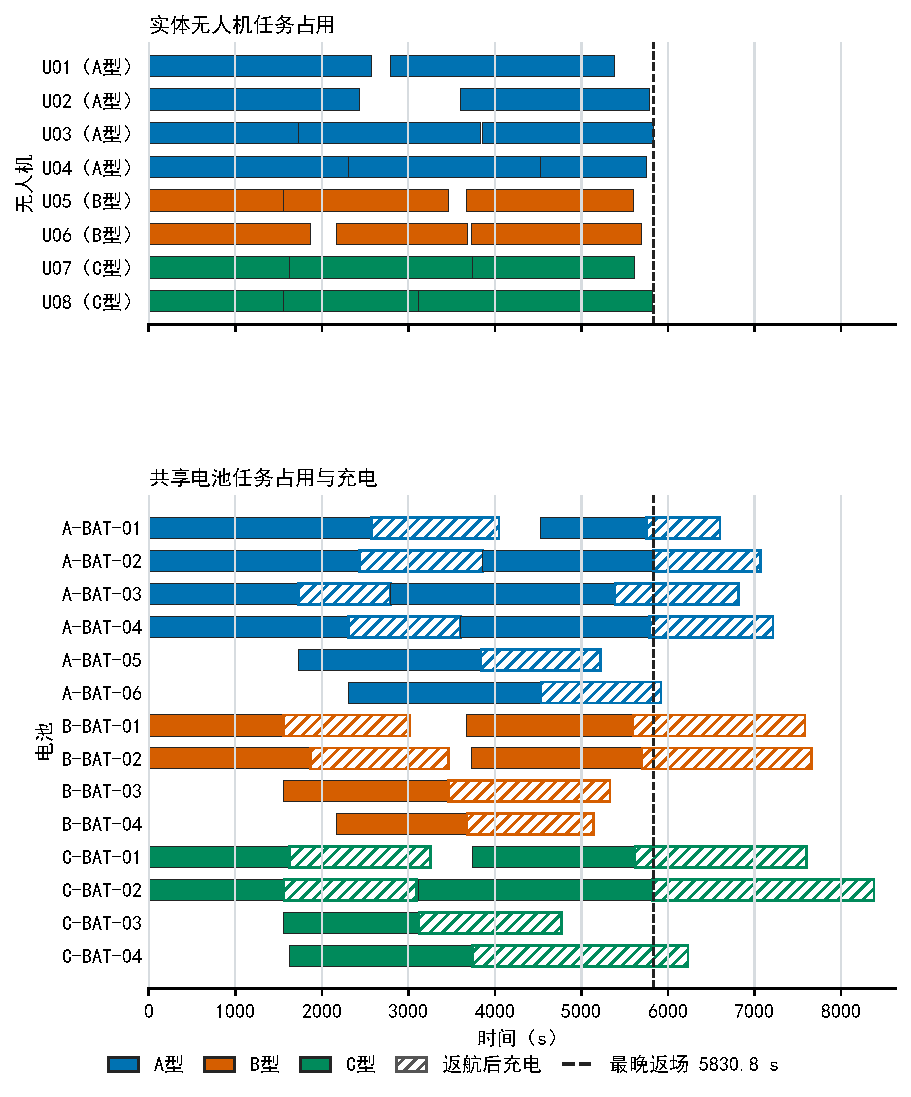
\includegraphics[height=0.82\textheight,keepaspectratio]{figures/q2_drone_battery_gantt.pdf}
\caption{问题二实体无人机与共享电池资源排程}
\label{fig:q2-gantt}
\end{figure}
\begin{figure}[htbp]
\centering
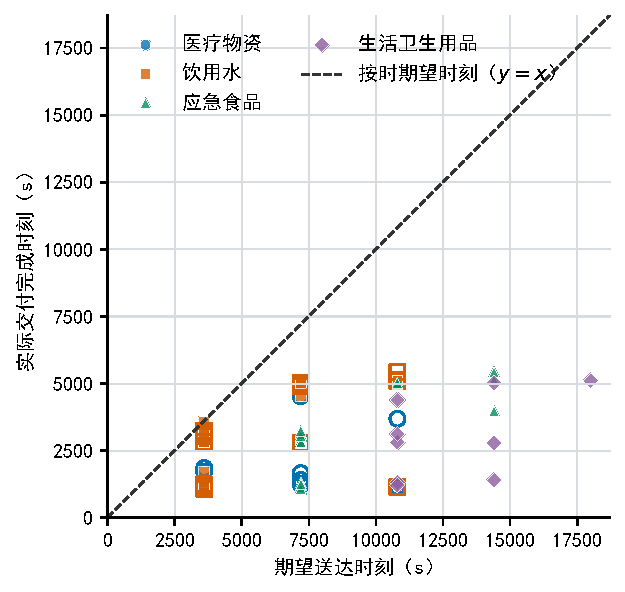
\includegraphics[width=0.82\textwidth]{figures/q2_expected_vs_actual_delivery.pdf}
\caption{货箱实际交付时刻与期望交付时刻对照}
\label{fig:q2-delivery}
\end{figure}
\clearpage
\subsection{独立可行性检验}

独立检查程序不读取求解器中间状态，而从导出的架次表和逐箱表重新构造所有航段。检查内容包括：80个货箱恰好出现一次；逐架次质量、体积、剩余载荷、能耗和返航SOC满足约束；逐箱交付时刻与路线递推一致；医疗及首批货箱全部满足硬时限；全部货箱不超过期望时刻；同一实体无人机任务区间无重叠；同一电池在上次返航并充至100\%后才可再次投入。新推荐方案通过全部检查；另外设置三个回归测试，核验等价类别定义、箱号还原与候选去重。该检验独立于调度算法，但沿用同一基础物理内核，不构成对能耗建模假设的独立实证验证。
